\section{FP4 --- Caractérisation du timbre vocal (MFCC)}
\label{sec:fp4}

Cette section couvre les exigences techniques \etref{5} (framing 256 samples / hop 128) et \etref{6} (matrice MFCC 62×13 sur 1 seconde d'audio).

\subsection{Objectif}

Calculer une signature spectrale compacte de la voix --- 13 coefficients cepstraux par tranche temporelle de 16 ms --- qui servira d'entrée au réseau de neurones de classification (FP6). La contrainte forte du projet est que tout le calcul tourne sur Cortex-M3 sans FPU : nous avons donc choisi une implémentation \textbf{intégralement Q15 fixed-point}, sans une seule instruction flottante.

\subsection{Conception}

\subsubsection{Pipeline en 8 étapes}

\begin{enumerate}
    \item \textbf{Préemphase} HPF du 1\textsuperscript{er} ordre : $y[n] = x[n] - 0{,}97 \cdot x[n-1]$. Constante Q15 : $\alpha_{Q15} = 31785$.
    \item \textbf{Découpage en 62 frames} de 256 échantillons avec recouvrement 50\,\% (hop 128). Le dernier frame est complété par 64 zéros.
    \item \textbf{Fenêtrage Hamming} via LUT précalculée 256 valeurs Q15 en flash.
    \item \textbf{FFT 256 points} radix-2 in-place avec scaling \texttt{>>~1} systématique à chaque étage (8 étages, perte cumulée $\sim$8 bits = précision suffisante pour la dynamique vocale 40 dB).
    \item \textbf{Magnitude au carré} sur les 128 premiers bins (symétrie hermitienne) : $P[k] = re^2 + im^2$.
    \item \textbf{Banc de 26 filtres MEL} triangulaires entre 0 et 4 kHz, espacés selon l'échelle perceptive mel.
    \item \textbf{$\log_2$ Q15 via LUT} : combinaison \verb|__builtin_clz| pour l'exposant + table de 1024 entrées + interpolation linéaire pour la mantisse normalisée.
    \item \textbf{DCT-II 26 → 13} avec matrice cosinus précalculée Q15 en flash.
\end{enumerate}

\subsubsection{Choix d'architecture}

\textbf{Bibliothèque séparée \texttt{lib/mfcc/}} : isole le code MFCC du firmware principal, facilite les tests unitaires et la réutilisation. API publique unique \texttt{compute\_mfcc()}, le reste est interne.

\textbf{Q15 strict bout en bout} : justifié par le besoin de garder du budget CPU pour FP6 (inférence CNN également gourmande en MAC). L'argument fort du projet : \emph{la chaîne de traitement audio numérique tourne intégralement en arithmétique entière sur un Cortex-M3 sans FPU}.

\textbf{Tables Q15 partagées C++/Python} : un script unique \verb|scripts/gen_tables.py| produit \verb|lib/mfcc/src/tables.cpp| et \verb|scripts/mfcc_tables.py|. Garantit que le firmware et le miroir Python utilisent exactement les mêmes constantes, condition nécessaire pour la validation bit-exact.

\subsubsection{Intégration dans la FSM FP3}

La FSM FP3 existante (\texttt{IDLE} $\rightarrow$ \texttt{ARMING} $\rightarrow$ \texttt{DUMPING}) est étendue avec deux nouveaux états :

\begin{itemize}
    \item \texttt{COMPUTING\_MFCC} : appel bloquant à \verb|compute_mfcc()| ($\sim$17 ms à 84 MHz).
    \item \texttt{DUMPING\_MFCC} : transmission série non-bloquante de la matrice 62×13 (1612 octets), magic header \verb|0xCAFEBABE|, footer \verb|0xC0DEBABE|.
\end{itemize}

Avant le calcul, \verb|adcBuffer| est flushé (\verb|bufTail = bufHead|) pour éviter un débordement pendant les 17 ms bloquantes. Sans flush, l'ISR à 32 kHz produirait $\sim$544 samples alors que le buffer en fait 512.

\subsection{Implémentation}

\subsubsection{Coût mémoire FP4}

\begin{table}[H]
\centering
\small
\begin{tabularx}{0.85\linewidth}{@{}l r X@{}}
\toprule
\textbf{Ajout} & \textbf{Taille} & \textbf{Persistance} \\
\midrule
\texttt{mfccMatrix[62][13]} \texttt{int16} & 1 612 octets  & persistant (consommé par FP6) \\
Buffers scratch FFT (real, imag) & 1 024 octets  & scope frame \\
Magnitude², mel\_energies, log\_mel & 668 octets    & scope frame \\
\midrule
Total RAM nouveau & $\sim$3.3 Ko & \\
RAM totale après FP4 & \textbf{27 392 octets} & \textbf{27,9\,\%} \\
Marge restante pour FP6 & $\sim$70 Ko & \\
\bottomrule
\end{tabularx}
\caption{Bilan mémoire FP4. La préemphase est appliquée \emph{in-place} sur \texttt{captureBuffer}, donc pas de duplication des 16 Ko audio.}
\end{table}

\subsubsection{Coût flash}

\begin{table}[H]
\centering
\small
\begin{tabularx}{0.85\linewidth}{@{}l r@{}}
\toprule
\textbf{Donnée constante} & \textbf{Taille} \\
\midrule
\texttt{HAMMING\_LUT[256]} & 512 octets \\
\texttt{TWIDDLE\_COS[128]} + \texttt{TWIDDLE\_SIN[128]} & 512 octets \\
\texttt{MEL\_FILTERS[26]} & $\sim$640 octets (struct fixe \texttt{coefs\_q15[20]}) \\
\texttt{LOG2\_LUT[1024]} + \texttt{LOG2\_SLOPES[1024]} & 4 Ko \\
\texttt{DCT\_Q15[13][26]} & 676 octets \\
Code MFCC compilé & $\sim$3-4 Ko \\
\midrule
Total flash nouveau & $\sim$9-10 Ko \\
Flash totale après FP4 & 6,6\,\% (34 812 octets) \\
\bottomrule
\end{tabularx}
\caption{Bilan flash FP4. Marge $>$93\,\% pour FP6.}
\end{table}

\subsubsection{Budget temps}

\begin{table}[H]
\centering
\small
\begin{tabularx}{0.6\linewidth}{@{}l r@{}}
\toprule
\textbf{Étape} & \textbf{Coût (62 frames)} \\
\midrule
Préemphase & 100 µs \\
Hamming & 200 µs \\
\textbf{FFT} & \textbf{15 ms} \\
Magnitude² & 300 µs \\
Banc MEL & 300 µs \\
$\log_2$ via LUT & 1 ms \\
DCT-II & 300 µs \\
\midrule
\textbf{Total \texttt{compute\_mfcc()}} & \textbf{$\sim$17 ms} \\
\bottomrule
\end{tabularx}
\caption{Budget temps estimé. Imperceptible côté UX dans la chaîne globale 1.72 s par appui bouton.}
\end{table}

\subsection{Validation (ET5, ET6)}

\subsubsection{Stratégie : miroir Python bit-exact}

La validation principale est un \textbf{test bit-exact} entre le firmware et un miroir Python (\verb|scripts/mfcc_reference.py|) qui réimplémente strictement le même pipeline Q15 (avec \verb|numpy.int16|). Les deux implémentations partagent les mêmes LUTs (générées par \verb|scripts/gen_tables.py|).

\begin{lstlisting}[language=Python, caption={Test bit-exact firmware ↔ Python}]
firmware = np.load("recording.mfcc.npy")
reference = compute_mfcc(load_wav("recording.wav"))
assert np.array_equal(firmware, reference)
\end{lstlisting}

Le critère est strict : \emph{0 différence sur les $62 \times 13 = 806$ valeurs}.

\subsubsection{Résultats}

\TODO{Capture du résultat du test \texttt{scripts/test\_mfcc\_integration.py --firmware} sur 3 audios test (sin\_1khz, silence, white\_noise) avec sortie ``[OK] BIT-EXACT match''. Fichier \texttt{assets/FP4/test\_bit\_exact\_output.txt}.}

\begin{figure}[H]
\centering
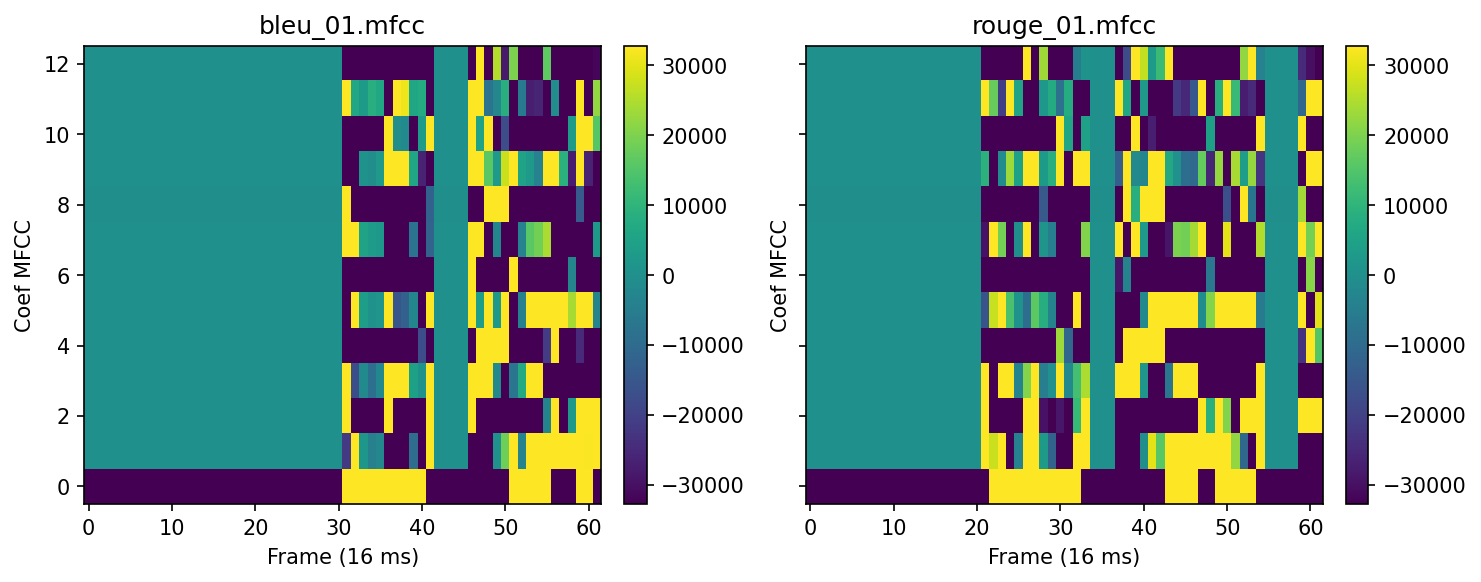
\includegraphics[width=0.85\linewidth]{figures/mfcc_heatmap_bleu_vs_rouge.png}
\caption{Matrice MFCC 62×13 pour les mots « bleu » et « rouge » prononcés. Les motifs visuellement distincts confirment que les MFCCs capturent assez d'information discriminante pour la classification CNN à venir (FP6).}
\label{fig:mfcc-heatmap}
\end{figure}

\subsection{Bilan FP4}

\begin{itemize}
    \item \textbf{Pipeline 100\,\% Q15} de bout en bout, validé bit-exact contre un miroir Python.
    \item \textbf{Coût total 17 ms} par enregistrement (FFT dominante à 15 ms), invisible côté UX.
    \item \textbf{Mémoire} : 27,9\,\% SRAM, 6,6\,\% flash --- très large marge pour FP6.
    \item \textbf{Tables partagées} générées par un script Python unique : aucune divergence possible entre les deux implémentations.
    \item \textbf{ET5} (framing 256/hop 128) et \textbf{ET6} (matrice 62×13) validées par construction et par test d'intégration.
\end{itemize}

\newpage
